\section{Experimental Evaluation}
\label{sec:evaluation}

This section aims to answer the following research questions: 

\begin{itemize}
\item \textbf{Performance:} How is \NM{}'s performance on synthetic benchmarks and real applications, comparing to popular allocators and NUMA-aware allocators? (Section~\ref{sec:performance}) 
\item \textbf{Memory Consumption:} What is the memory consumption of \NM{}? (Section~\ref{sec:memory})
\item \textbf{Scalability:} How is the scalability of \NM{}? (Section~\ref{sec:scale})
\item \textbf{Design Decisions:} How important design choices can actually affect the performance? (Section~\ref{sec:design})	
\end{itemize}

\subsection{Experimental Setup}
\NM{} was evaluated on two different machines, as specified in Table~\ref{table:Machine}. Typically, machine A has 2 nodes, with 40 cores in total, while machine B has 8 nodes with 128 cores. For machine B, any two nodes are less than or equal to 3 hops. For the evaluation, both machines turned off the hyperthreading. For the performance data, all data shown in this paper is the average of 10 runs, in order to avoid any bias caused by unexpected events.  

\begin{table}[!ht]
 \centering
  \footnotesize
  \setlength{\tabcolsep}{1.0em}
\begin{tabular}{c | c | c}
\hline
System & \textbf{Machine A} & \textbf{Machine B} \\ \hline
CPUs/Model & Xeon Gold 6138	& Xeon(R) Platinum 8153\\ \hline
CPU Frequency & 2.10GHz & 2.00GHz\\ \hline
NUMA Nodes & 2 & 8 \\ \hline
Physical Cores & 2$\times$20 & 8$\times$16 \\ \hline
Node Latency & \specialcell{local: 1.0 \\ 1 hop: 2.1} & \specialcell{local: 1.0 \\ 1 hop: 2.1 \\ 2 hops: 3.1}\\ \hline
Interconnect Bandwidth & 8GT/s & 10.4GT/s\\ \hline
Linux & Ubuntu 18.04 & Debian 10\\ \hline
Compiler & GCC-7.5.0 & GCC-8.3.0 \\ \hline
%Memory Bandwidth & 19.87 GB/s & \\ \hline
  \end{tabular}
   \caption{Machine Specifications.\label{table:Machine}}
  \vspace{-0.4in}
\end{table}


\subsection{Performance Evaluation}

\label{sec:performance}

In order to evaluate the performance, we employ both synthetic applications (in Section~\ref{sec:scale}) and real applications on two different machines, where all are multithreaded applications. The number of threads is set to the the total number of cores on two machines if possible, with 40 threads in machine A and 128 threads in machine B. For applications with multiple phases (e.g., \texttt{ferret} and \texttt{dedup}) or works only for power-of-two threads, we chose the maximum number of threads that is smaller than but is close to the total number of cores.  We compare \NM{} with multiple popular allocators, such as default Linux Allocator, TcMalloc-2.7~\cite{tcmalloc}, NUMA-Aware TcMalloc~\cite{tcmallocnew}, jemalloc-jemalloc-5.2.1~\cite{jemalloc}, Intel TBB--2020.1~\cite{tbb}, and Scalloc-1.0.0~\cite{Scalloc}. For the simplicity, NUMA aware TcMalloc is called as TcMalloc-NUMA in the remainder of this paper. The performance data is using the normalized runtime, by normalizing the runtime of each allocation to the runtime of Linux's default   allocator. That is, the lower bar indicates a better performance. In the remainder of this paper, all performance data are using the same format. 

For real applications, we evaluated on all applications from the PARSEC suite~\cite{parsec}, and seven real applications like \texttt{Apache httpd-2.4.35}, \texttt{MySQL-5.7.15}, \texttt{Memcached-1.4.25}, \texttt{SQLite-3.12.0}, \texttt{Aget}, \texttt{Pfscan}, and \texttt{Pbzip2}. 
The inputs for these applications are listed as follows. PARSEC applications are using native inputs~\cite{parsec}. For MySQL, we use \texttt{sysbench} with 40 and 128 threads separately, each issuing 100,000  requests. The \texttt{python-memcached} script is used for \texttt{Memcached}, with 3000 loops to get the sufficient runtime~\cite{memcached}. The  \texttt{ab} is used to test \texttt{Apache} server~\cite{apachetest}, by sending 1,000,000 requests. \texttt{Aget} is tested  by downloading a 30 M file, and \texttt{Pfscan} is tested by searching  a keyword in a 500M data. In terms of \texttt{Pbzip2}, we test it by compressing 10 files with 30M each. Finally, SQLite is tested through a program called \texttt{threadtest3}~\cite{sqlitetest}. 

%In the Hoard~\cite{Hoard} benchmarks, we used 100 iterations and 1,280,000 64-byte objects for threadtest and also we run larson for 10 seconds with 1,000 7-2048 bytes object to cover all size classes in almost all allocators for 10,000 iterations.For false sharing , we used 100,000 inner-loop , 100,000 iterations with 8 bytes objects. 

%The number of threads of all benchmarks were adjusted according how many cores and nodes in the target machine to make threads could be properly distributed over the nodes and cores, making the number of threads as close as the number of cores. Mostly, thread number was 40 in the Machine A and 128 in the Machine B, and I will give the specific number below if it is not this default value. 
The normalized performance runtime of different allocators on Machine A an on Machine B can be seen in Fig.~\ref{8node-parsec-perf} and Fig.~\ref{2node-parsec-perf} separately,  where all data is normalized to the runtime of the default Linux allocator. By default, \NM{} will embed with the interleaved heap support. However, two applications, \texttt{canneal} and \texttt{raytrace}, have  a much worse performance when the interleaved heap is enabled, since both of them spend a large portion of their time (over 62\% and 82\%) in the serial phase (before creating any child thread). Since the interleaved heap indicates that the allocations can be satisfied in remote NUMA nodes, this design may lead to a large number of remote accesses for the serial phase. Thus, these two figures show the best data for two applications, without the support of interleaved heap. We further discuss the pros and cons of using interleaved heap in Section~\ref{sec:interleavedheap}.  


\begin{figure}[H]
    \centering
    \begin{subfigure}{0.9\textwidth}
    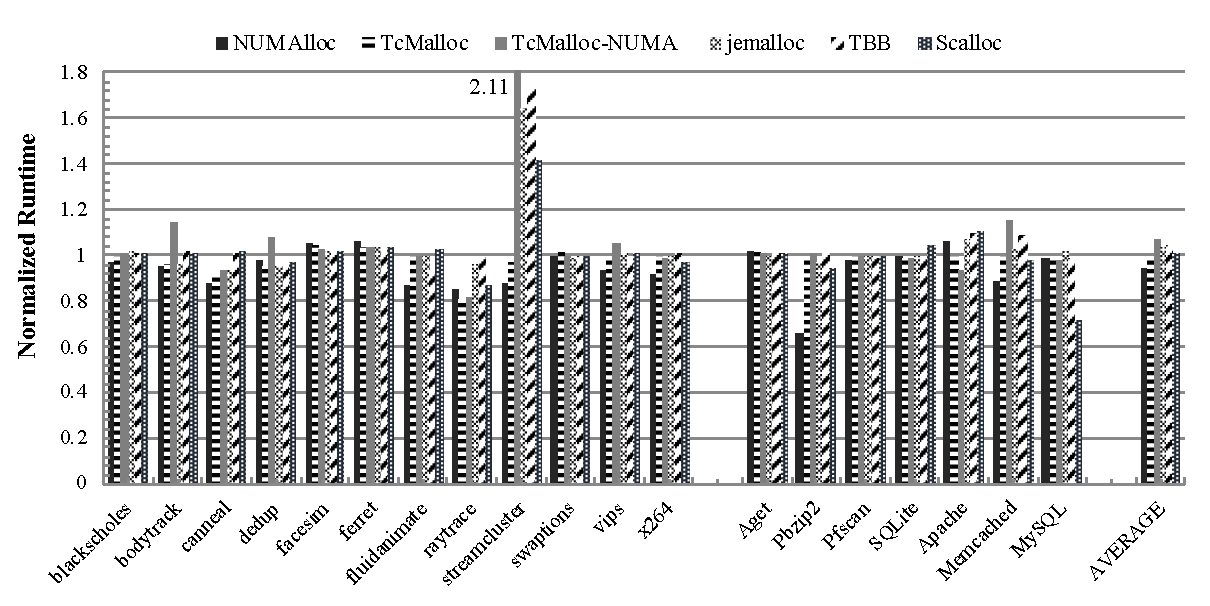
\includegraphics[width=\textwidth]{figure/2-node-parsec-perf.pdf}
    \caption{Machine A (2-Node)\label{2node-parsec-perf}}
    \end{subfigure}
    
	\vspace{0.1in}  
	
	\begin{subfigure}{0.9\textwidth}    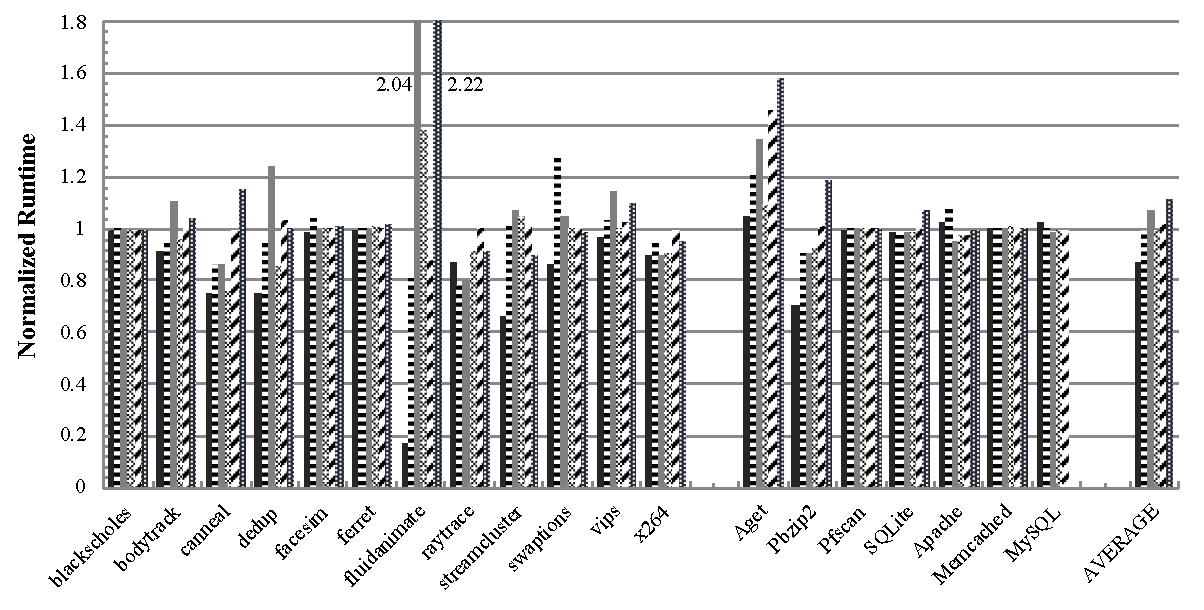
\includegraphics[width=\textwidth]{figure/8-node-parsec-perf.pdf}
    \caption{Machine B (8-Node)\label{8node-parsec-perf}}
    \end{subfigure}
    \caption{Performance with different allocators, where all data are normalized the default Linux allocator. \label{sec:perf}}
 \end{figure}


Overall, \NM{} has the best performance on two machines. Comparing to the default allocator, \NM{} is 6\% faster on Machine A and 13\% faster on Machine B. TcMalloc is the second best one among all allocators, which is only 1\% faster than that of the default allocator. \NM{} is actually much faster than the other NUMA-aware allocator -- TcMalloc-NUMA~\cite{tcmallocnew}. For the best case (e.g., \texttt{fluidanimate}), \NM{} is running up to  $5.8\times$ faster than the default Linux allocator, and it is $4.7\times$ than the second best one--TcMalloc. We also notice that \NM{} achieves a much better performance on the machine with more hardware cores and more NUMA nodes, which indicates \NM{}'s scalable design. 

The default Linux allocator achieves a reasonable performance on the NUMA architecture due to its arena-based design. Based on our analysis, the Linux allocator will always return an object back to its original arena, and then allocate such objects to the thread owning this arena afterwards. This design is integrating well with Linux's first-touch allocation policy, which essentially avoids the owner shifting issue of most allocators. By default, Linux utilizes the first-touch policy to manage the physical memory~\cite{Lameter:2013:NO:2508834.2513149}, which a page is allocated in the same node as the thread that first touches it. Therefore, an object is typically allocated from the local node of its allocation thread, since it typically accesses this object after the allocation. Objects that are deallocated from a different thread will be always returned back to its original arena, and then will be re-utilized by its original allocation thread locally. In contrast, other allocators typically utilize a per-thread cache to store objects that are deallocated by the current thread, which may lead to remote accesses unnecessarily in a NUMA architecture when the deallocation thread is located in a different node from the allocation thread, causing the ``owner shifting'' issue.  

 TcMalloc-NUMA is the only available allocator that is claimed to support the NUMA architecture~\cite{tcmallocnew}. However, its performance is not good, which is even slower than that of TcMalloc. TcMalloc-NUMA is based on TcMalloc-0.97 (released in 2008), which does not have many new features of TcMalloc-2.7 (the version for our evaluation). TcMalloc-NUMA imposes the largest overhead \texttt{fluidanimate} ($2.04\times$) on the Machine B (8-node), due to without the thread binding support.  Based on our understanding, although it achieves node-aware memory management, it does not implement following mechanisms of \NM{}, including topology-aware task assignment, interleaved heap, automatic huge page support, and efficient object migration. We examine the performance impact of these mechanisms further in Section~\ref{sec:design}.    
  


%We  can see that the average value of \NM{} is 0.97 in Machine A and 0.92 in Machine B and it is always the best among all other allocators. The reason that \NM{} got better performance in Machine B is that there are more nodes and more cores in Machine B, which means \NM{} could be very helpful to better to take use hardware resource of multi nodes and cores. but we could get amazing improvement if we shutdown interleaved heap in \NM{} and we will give the data in following sections.In the figure ~\ref{8node-parsec-perf}, we could see more exciting improvement from \NM{}, with average normalized value of 0.92 that is not only the best but also far aware better than all the rest allocators that TcMalloc and jemalloc got 0.99, TcMalloc-NUMA and TBB got roughly 1.07 and 1.01 separately. And also, we can see that the performance of \NM{} is the best for almost each single applications, especially it got 0.17 in fluidanimate and 0.66 in streamcluster which is far better than any of other allocators. As the same thing, the performance of ratrace and canneal is not good here, we will talk about it later after we shut down the interleaved heap.


%In the figure ~\ref{hoard-perf}, we show the normalized performance for Hoard benchmarks in Machine A and Machine B separately. We can see from figure ~\ref{hoard-perf} that the average value of \NM{} is also the best, which is 0.47 that means 2 times faster than default Linux Allocator, and jemalloc got 0.7 and Scalloc got 0.9. In the threadtest, the normalized value of \NM{} is 0.19 , far better than any of others, which means there are few central free list competitions, mainly contributed by properly node management and low overheads operations. For false sharing, \NM{}'s performance is also almost the best as same as Scalloc and jemalloc, which means they could handle false sharing issues very properly. In the larson, \NM{} and TcMalloc are the best, which mainly contributed by their low overheads for allocation and remote de-allocation, but due to our better node management, \NM{} could be better in the Machine B which will be mentioned later. In the figure ~\ref{hoard-perf}, we can also see that \NM{} got lowest average normalized value:0.33, significantly smaller than any of others that TBB got 0.99, Scalloc and jemalloc got roughly 1.14. And also, \NM{} and Scalloc could handle false sharing issue very well, and \NM{} could extremely well reduce central free list competition in threadtest. In larson, \NM{} is the best due to its properly multi-node management. 


\subsection{Memory Consumption}
\label{sec:memory}

We also measured the maximum memory overhead of different allocators for these applications. For non-server applications, such as \texttt{Aget}, \texttt{Pbscanf}, \texttt{PbZip2} and all PARSEC applications, we utilized the sum of the maxresident output from the time utility and the size of huge pages, since the time output does not include the usage of huge pages. In order to determine the huge page usage, a script is used to periodically collect the number of huge pages by reading from \texttt{/proc/meminfo} file, and then the maximum value of huge pages are used. Memory assumption of server applications, such as \texttt{MySQL}, \texttt{SQLite}, and \texttt{Memcached}, \texttt{Apache}, is collected by the sum of both \texttt{VmHWM} and \texttt{HugetlbPages} fields from \texttt{/proc/PID/status} file, after the corresponding client exits. 
%We always reboot server applications for each single test. 

%\end{comment}

%\renewcommand{\arraystretch}{1.5}
\begin{table}[tp]
\footnotesize
	\setlength{\tabcolsep}{0.3em}
  \centering
    \begin{tabular}{|l|r|r|r|r|r|r|r|}
    \hline
    \multirow{2}{*}{Apps}&
    \multicolumn{7}{c|}{Memory Usage (MB)}\\
    \cline{2-8}
    &Linux&\NM{}&TcM&TcM-N&jem&TBB&Scalloc \\ \hline
    \hline
    blackscholes&615&509&621&623&633&615&630\\ \hline
    bodytrack&37&161&45&46&570&37&1994\\ \hline
    canneal&888&879&774&757&1294&888&36149\\ \hline
    dedup&912&1236&983&1023&1389&912&8556\\ \hline
    facesim&560&500&603&601&1133&547&3056\\ \hline
    ferret&184&493&195&183&596&184&3377\\ \hline
    fluidanimate&470&392&483&484&481&470&3437\\ \hline
    raytrace&1288&1472&1092&1543&1287&1288&4398\\ \hline
    streamcluster&113&105&123&121&127&113&193\\ \hline
    swaptions&33&268&16&21&540&37&1817\\ \hline
    vips&228&536&248&269&778&227&3681\\ \hline
    x264&2859&2721&3047&3064&3719&2859&5402\\ \hline \hline  
    Aget&8&74&11&10&93&8&80 \\ \hline
    Apache&8&34&10&9&10&4&42\\ \hline
    Memcached&16&80&25&24&41&18&263\\ \hline
    Mysql&277&732&314&315&500&276& N/A \\ \hline
    Pbzip2&463&747&817&813&1121&454&4881 \\ \hline
    Pfscan&522&542&528&528&535&522&554\\ \hline
    Sqlite3&45&284&60&75&139&44&681 \\ \hline
    \hline
    Total&{\bf 9527}&{\bf 11763}&{\bf 9993}&{\bf 10510}&{\bf 14986}&{\bf 9502}&{\bf 79190}\cr\hline
    \end{tabular}
  \caption{Memory consumption of different allocators. Here, TcM stands for TcMalloc, TcM-N is TcMalloc-NUMA, and jem is jemalloc. \label{tab:memory_consumption}}
\end{table}


The memory overhead of different allocators is listed in Table~\ref{tab:memory_consumption}, which is running on Machine B. We chose Machine B, because it has more nodes and physical cores. Then it is better to see the scalability of an allocator. In total, \NM{}'s memory consumption is around 23\% more than that of the default Linux allocator. For applications with small footprint, \NM{} may utilize up to $9.3\times$ more memory, such as \texttt{Aget}. Intel TBB allocator has the smallest memory consumption, and the default Linux allocator is the second best one. Scalloc is the worst one in terms of memory consumption, which consumes around  $8.3\times$ more memory that that of TBB.  
 
 Based on our analysis, the following reasons may lead to \NM{}'s more memory consumption. The Linux will utilize huge pages by default in machine B, if a memory area is larger than the size of a huge page (2MB). Since \NM{} utilizes \texttt{mmap} to allocate a huge chunk of virtual memory, this makes all heap memory for real objects will be allocated from huge pages. Currently, \NM{} also utilizes 1MB as the superblock for each size class, making objects of a size class that will occupy at least 1MB. Therefore, an application with many size classes will waste more memory.  
 
 Scalloc has excessive memory consumption, since its design does not support transparent huge pages very well. Similar to \NM{}, Scalloc utilizes a \texttt{mmap} system call to allocate a continuous huge region of virtual memory from the underlying OS. Thus, the OS will utilize huge pages for any memory usage from such a region, when transparent huge pages are enabled by default. Coincidentally, every thread will get a virtual span (2MB) for each size class, even if only one object is allocated from a size class. This indicates that each size class of each thread will utilize 2MB physical memory at least, even if only one object is used.  Differently, \NM{} supports transparent huge pages in its design, as described in Section~\ref{sec: others}.
 
\begin{comment}


In Fig.~\ref{2node-hoard-mem}, the average normalized value of \NM{} is larger than others, but actually not too much, which is 2.3 for \NM{}, 1.9 for TcMalloc-NUMA and 1.8 for TcMalloc. It is because that proper node management is utilized in \NM{} and also in TcMalloc-NUMA, so that each node also preserves some memory not only thread locals.But we believe that this little more memory overheads are totally acceptable. It is also the same thing for Fig. 10, that the average value for \NM{} is little higher than others, which is 5.3. But in this 8 nodes machine, numalloc is not the worst, that Scalloc's average value is 25 and jemalloc is 9.4. One main reason that the value of \NM{} is smaller is that we use mini size bags in \NM{} which is less than the size of one page for small objects and also memories for small objects are shared per node but per cores in Scalloc.
	
\end{comment}


\subsection{Scalability}
\label{sec:scale}

In order to evaluate the scalability of \NM{}, we evaluate the following configurations on the Machine B: 8 threads on one node (called as 8T1N), 16 threads on one node (16T1N) and two nodes (16T2N), 32 threads on two nodes (32T4N) and 4 nodes (32T4N), 64 threads on two nodes (64T4N) and 4 nodes (64T8N), and 128 threads on 8 nodes (128T8N). Machine B is chosen since it has more cores and more nodes. \NM{}'s performance on these configurations is shown in Fig.~\ref{fig: numalloc-scalability}. For some applications, such as \texttt{facesim}, \texttt{ferret}, \texttt{fluidanimate}, \texttt{streamcluster}, \texttt{swaptions}, \NM{} scales very well. Some applications, such as \texttt{blackscholes}, \texttt{raytrace}, or \texttt{x264}, are not scalable very well. Due to the space limitation, we did not show the results of the Linux allocator, but they share the similar trend. We also observe that \NM{} typically performs better with the lower number of nodes, on a given number of threads.  This indicates that a lower number cores enables a better share of data among different threads. 

\begin{figure}[!h]
    \centering
    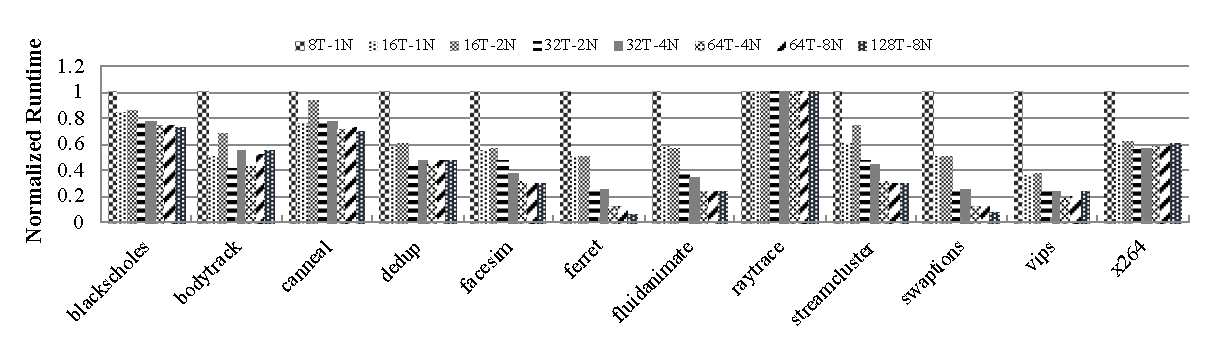
\includegraphics[width=\textwidth]{figure/scalobility-numalloc.pdf}
    \caption{Scalability of \NM{} with different configurations on Machine B (8-Node), where the data are normalized to 8T1N.\label{fig: numalloc-scalability}}
\end{figure}

\begin{figure}[!h]
    \centering
    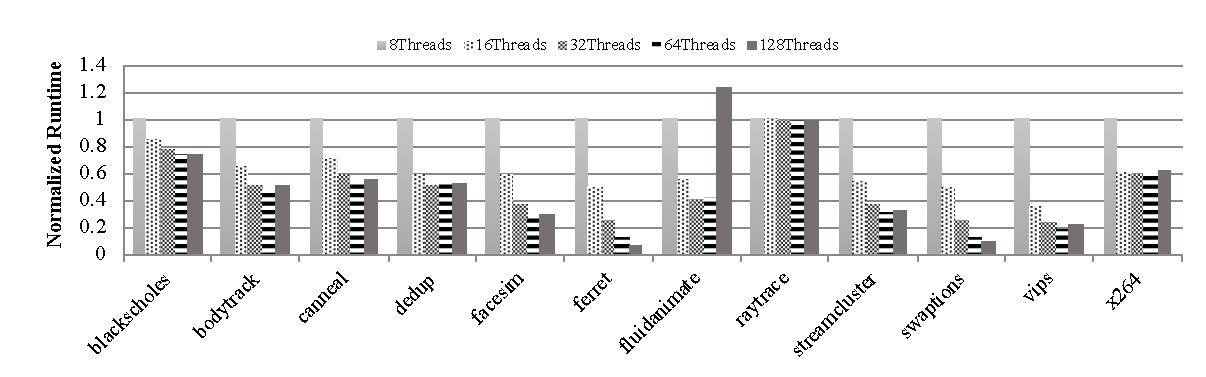
\includegraphics[width=\textwidth]{figure/scalability-pthread.pdf}
    \caption{Scalability of the Linux's default allocator on Machine B (8-Node), where the data are normalized to 8Threads.}
    \label{pthread-scalibity}
\end{figure}

 In order to understand the scalability of \NM{} when comparing to other allocators, we also evaluate them with synthetic applications from Hoard~\cite{Hoard}, including \texttt{threadtest}, \texttt{larson}~\cite{Larson}, \texttt{cache-scratch} and \texttt{cache-slash}, which is also employed by existing work~\cite{Scalloc}. . The reason of utilizing synthetic applications is that they were designed to be scalable~\cite{Scalloc}. Therefore, we could eliminate the scalability issue caused by applications. Since other allocators cannot specify the configuration, we only evaluate the scalability with different number of threads. For \NM{}, we maximize the number of threads on each node. For instance, the result of 32 threads will use 2 node, since each node has 16 cores. The corresponding data is shown as Fig.~\ref{sythentic-scalability}. 
 
\begin{figure}[!ht]
    \centering
    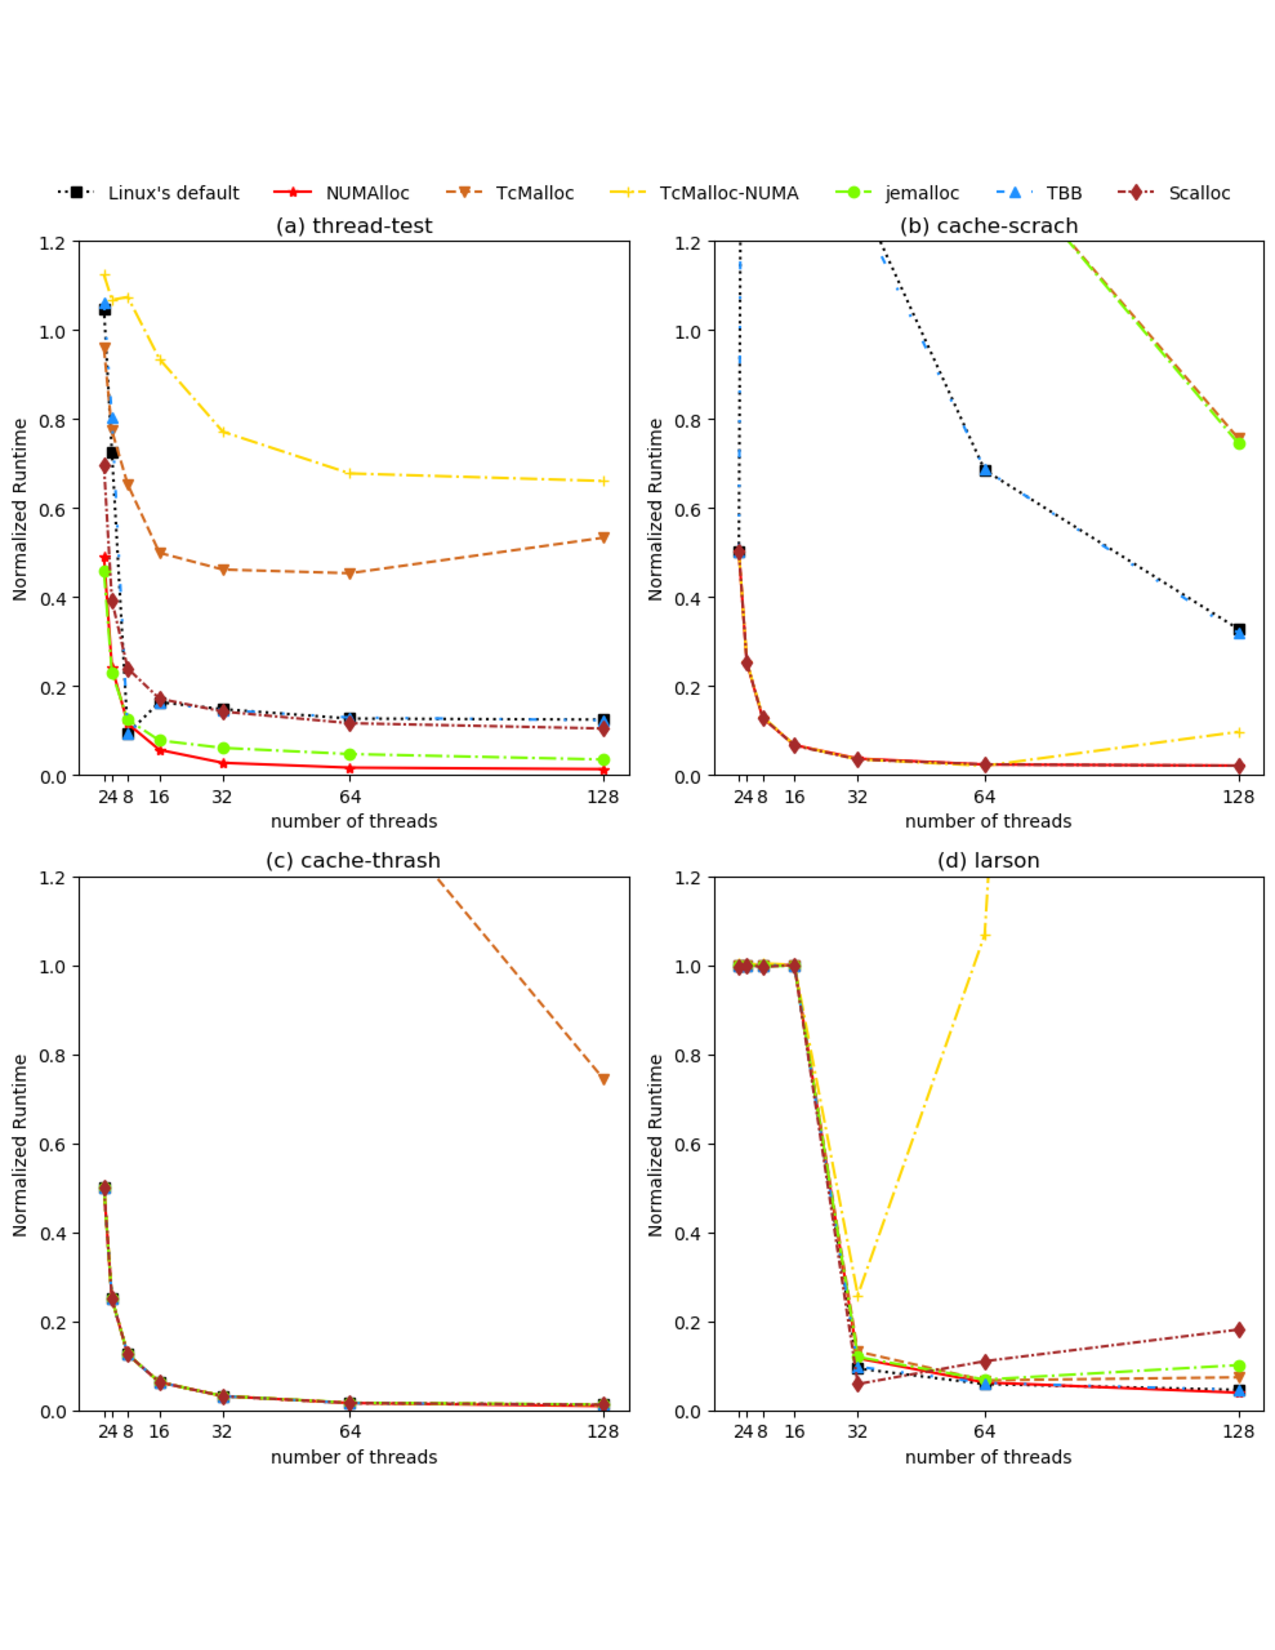
\includegraphics[width=\textwidth]{figure/sythentic-scalobility.pdf}
    \caption{Scalability of different allocators\\  the data are normalized the runtime of the default Linux allocator with one thread.}
    \label{sythentic-scalability}
\end{figure}

Among these applications, \texttt{cache-scratch} tests passive false sharing, and \texttt{cache-thrash} tests active false sharing. False sharing occurs when multiple threads are concurrently accessing different words in the same cache line. 
Passive false sharing is introduced upon deallocations, where the reallocation of freed objects introduces the false sharing. In contrast, active false sharing can be introduced during the first allocation of objects, where a thread is not responsible for allocating all continuous objects in the cache line. For these false sharing tests, we use 100,000 inner-loop, and 100,000 iterations with 8-byte objects. \NM{} will not introduce active false sharing, since each thread will get a page initially. 
 Although \NM{} might introduce passive false sharing in theory, due to its per-thread cache design, it avoids remote allocations across the node. Other allocators do not have such mechanisms. That is the reason why \NM{} is one of the best allocators for
 \texttt{cache-scratch} , and achieves much better speedup than all other allocators in \texttt{cache-thrash} (30\% faster than the second best one), as shown in Fig.~\ref{sythentic-scalability}.  

 \texttt{larson} is to simulate a multithreaded server that could respond to requests from different clients. Each thread  will receive a random number of objects in the beginning, perform a random number of allocation and deallocations to simulate the handler for processing requests, and then pass objects to the next thread. We test \texttt{larson} for 10 seconds with 1,000 objects for 10,000 iterations, where each allocation is between 7 bytes and 2048 bytes. As shown in Fig.~\ref{sythentic-scalability}, \NM{} is around 16\% faster than the second best allocator--TcMalloc--with 128 threads.   


\texttt{threadtest} is an application that performs a large number of allocations and deallocations with a specified number of threads. Also, it allows to specify how much work to be done between each allocation and deallocation. For \texttt{threadtest}, we use 100 iterations, 1,280,000 allocations, 0 work, and 64-byte objects (for the allocation).  This benchmark will stressfully test the performance overhead of allocation and deallocation. For this application, \NM{} is $2.6\times$ faster than the second best one (jemalloc), when there are 128 threads. %since every thread will has its own heap and it only imposes some when getting objects from the shared bag. But \NM{} obtains a number of objects at a time, at the page level, which significant reduce the possibility of contention. 


When the number of threads is equal to the number of cores (128), \NM{} has the best overall performance, and for almost all single applications. Overall, \NM{} is running 79\% faster than the second best one (Scalloc), and  $2.2\times$ faster than the default one on machine 2.  Multiple reasons contribute to the good performance of \NM{}:  \NM{} imposes very minimal system call overhead, and little synchronization overhead. Also, it introduces less remote accesses than all other allocators, due to its NUMA-aware design. 



%That is the reason why it has a good performance as the Linux allocator for \texttt{cache-thrash}.

 
\begin{comment}

\begin{figure}[!ht]
    \centering
    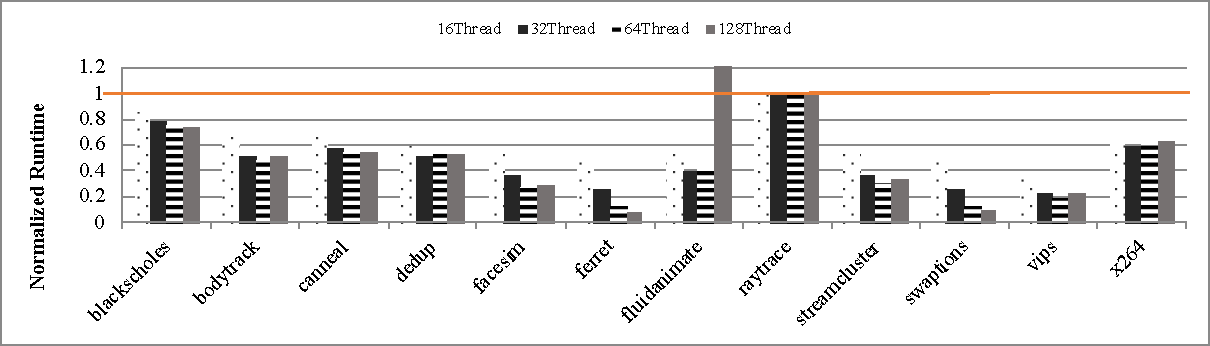
\includegraphics[width=\textwidth]{figure/scalobility-pthread.pdf}
    \caption{Normalized performance of Linux's default allocator without binding for PARSEC benchmarks in Machine B}
    \label{pthread-scalibity}
\end{figure}
We will evaluate the scalability on 8threads, 16threads, 32 threads, 64 threads and 128 threads. 
(one node, two node, four nodes, and 8 nodes). 
	
\end{comment}


\subsection{Design Choices}
\label{sec:design}

This section further confirms multiple design choices of \NM{}. Some mechanisms are very basic, such as node-aware memory allocation, which is mandatory for NUMA-aware memory allocators, and cannot be evaluated separately. Therefore, they are not evaluated here. Some design choices may only help on one or two applications, such as efficient objects migration. 
\subsubsection{Thread Binding}
\label{sec: threadbinding}

\begin{figure}[!h]
    \centering
    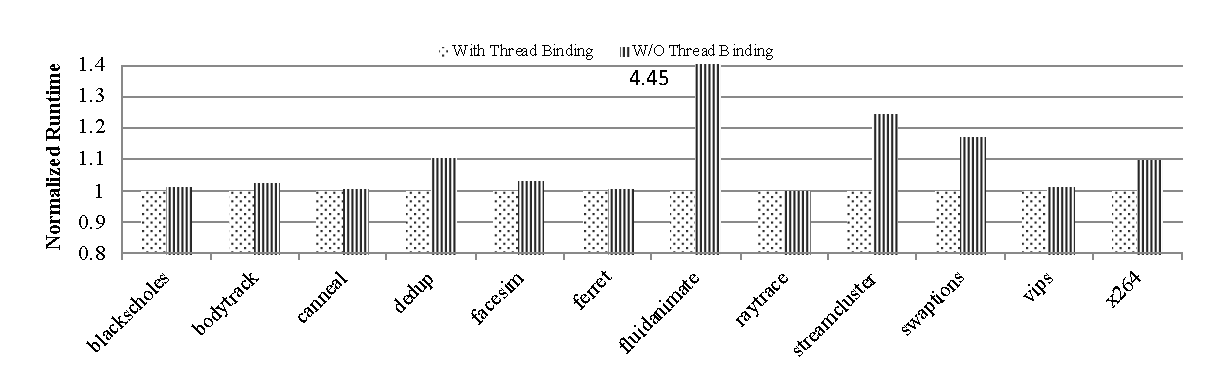
\includegraphics[width=\textwidth]{figure/WO-pthread-binding.pdf}
    \caption{Normalized runtime with and without thread binding on Machine B (8-Node) (using the Linux allocator)}
    \label{binding-pthread-scalibity}
\end{figure}

Fig.~\ref{binding-pthread-scalibity} shows performance difference with and without thread binding. \NM{} relies on thread binding, which can not be disabled explicitly. For this experiment, we utilize the default allocator, but designing a specific library to bind threads to different nodes in an round-bin way, similar to \NM{}'s thread binding policy. We observe that thread binding may achieve significant difference. \texttt{fluidanimate} runs around $5\times$ faster with the thread binding, while  \texttt{streamcluster} runs 20\% faster than the default one with the binding. This clearly indicates that thread binding benefits the performance. Based on our analysis, there are two reasons for this performance speedup. First, a thread will not be migrated to a different core, avoiding unnecessary remote accesses. Second, \NM{}'s thread binding helps load balance, thus reducing interconnect or memory controller congestion.


\subsubsection{Interleaved Heap} 
\label{sec:interleavedheap}

\begin{figure}[H]
    \centering
    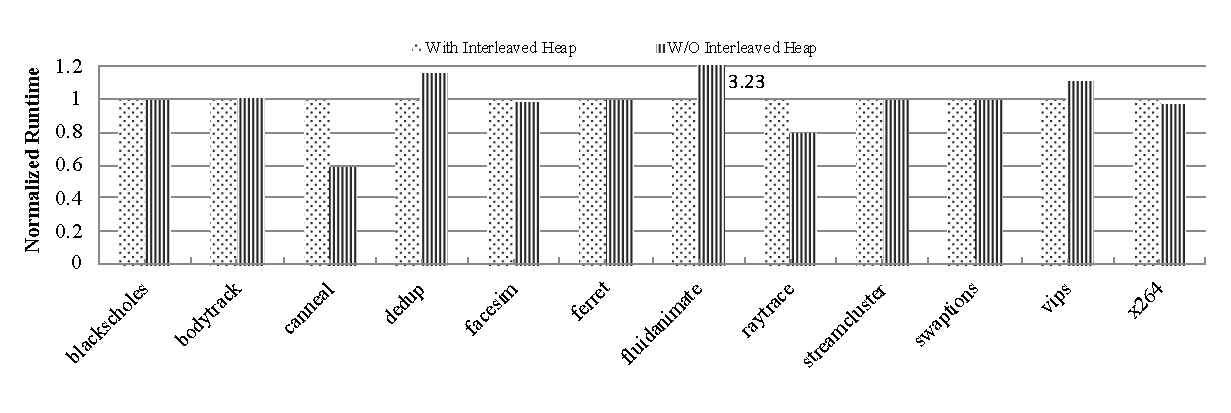
\includegraphics[width=\textwidth]{figure/interleavedheap.pdf}
    \caption{Normalized runtime with  and without interleaved heap on Machine B (8-Node).\label{fig:interleavedheap}}  
\end{figure}

We first evaluate the performance difference when the support of interleaved heap is enabled or not. As described in Section~\ref{sec:performance}, some applications, especially those ones having a large portion of time in the serial phase, may not have good performance with the interleaved heap support. The interleaved heap will allocate the memory from all nodes interleavedly, instead of from the local node (based on the default first-touch policy). The interleaved heap could be utilized to avoid load imbalance issue for shared objets. 

However, there are two issues for the interleaved heap. First, the allocator may not know whether an object is shared or not at the first time. Therefore, all objects that are allocated in the main heap (before creating any child thread) will be treated as the shared heap. However, a private object, if it is allocated interleavedly in multiple nodes, may introduce unnecessary overhead due to remote accesses. Second, some applications are spending too much time in the serial phase, where the interleaved heap cannot benefit the performance for the serial phase. 

The performance data with and without interleaved heap is shown in Fig.~\ref{fig:interleavedheap}. Note that we have evaluated all real applications listed in Section~\ref{sec:performance}. The applications that have no or little performance impact by the interleaved heap are omitted in this figure. From Fig.~\ref{fig:interleavedheap}, we have the following conclusion: the interleaved heap will benefit (or at least no harmful impact) the performance for most applications, except applications with a large portion of serial phase (e.g., \texttt{canneal} and \texttt{raytrace}). Some applications, such as \texttt{fluidanimate}, will have the performance speedup of $3.5\times$ with the interleaved heap. Therefore, the interleaved heap can be enabled by default, unless programmers know that it will not benefit the performance. A simple metrics is to use the portion of its serial phase. 


%figure ~\ref{parsec-no-interleaved-perf} we show some performance results of some applications that got significant different values after we shut down interleaved heap for \NM{}. We can see that for some applicatios with less data sharing between threads like ratrace and canneal, \NM{} could got significant improvements due to its low overheads and proper memory management. But for some other applications with intensive memory operations and sharing like fluidanimate, shutting down interleaved heap could hurt performance, since interleaved heap could help to distributed resource contention evenly over multi-nodes and then got low overheads.

\subsubsection{Huge Page Support} 
Since Machine B utilizes transparent huge pages by default, we evaluate the performance impact of huge page support on Machine A (2-node machine). We only utilize PARSEC applications for this evaluation. 

\begin{figure}[!h]
    \centering
    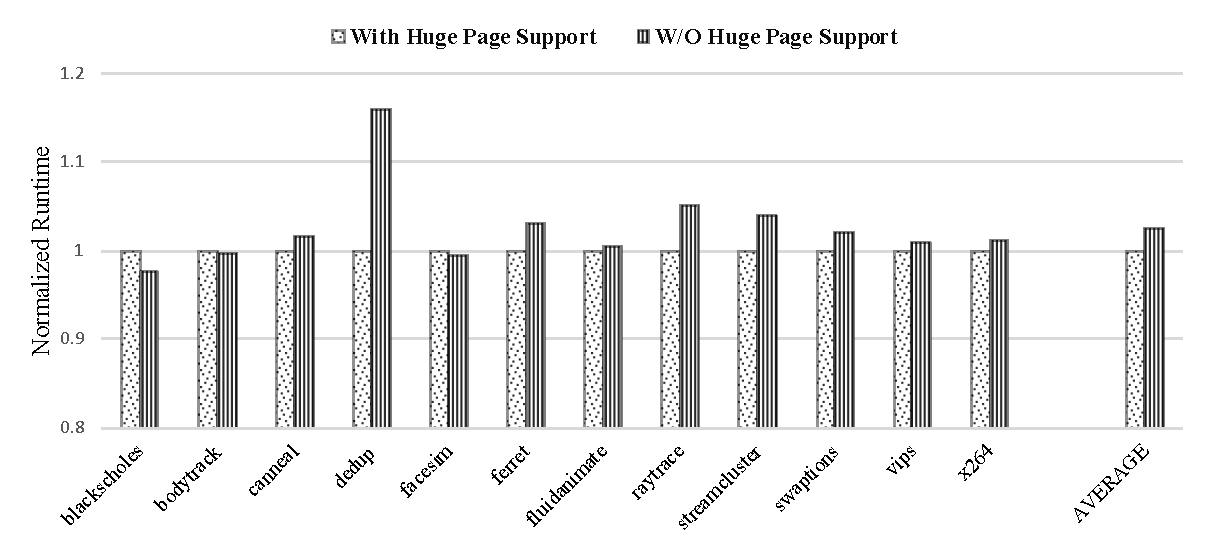
\includegraphics[width=\textwidth]{figure/hugepage.pdf}
    \caption{Normalized runtime with and without huge page support on Machine A (2-node).}
    \label{fig:hugepage}
\end{figure}

The results are shown in Fig.~\ref{fig:hugepage}. When integrating with huge page support, \NM{} achieves a significantly better performance for \texttt{dedup}, where the performance difference is around 15\%. On average,  the huge page support improves the performance of all evaluated applications about 2.5\%. This clearly indicates that it is beneficial to have huge page support integrated with the memory allocator.  


